\section{Implementation}\label{sec:impl}

The \tube system has two components; the tube itself and the screen. The tube is attached to an acrylic enclosure that houses a small Force-Sensing Resistor (FSR) and Inertial Measurement Units (IMU) that possesses 5 degree of freedom. The IMU captures the 3-dimensional motions of the tube and translate it into 2-dimensional movement in the screen. Additionally, it also records the angle in which the tube is rotated and how fast it is rotating. With the FSR integrated in the tube, how hard the user breathe into the tube is also captured. All of these informations will then be passed into arduino which will be read by a processing module.

\begin{figure}
  \centering
  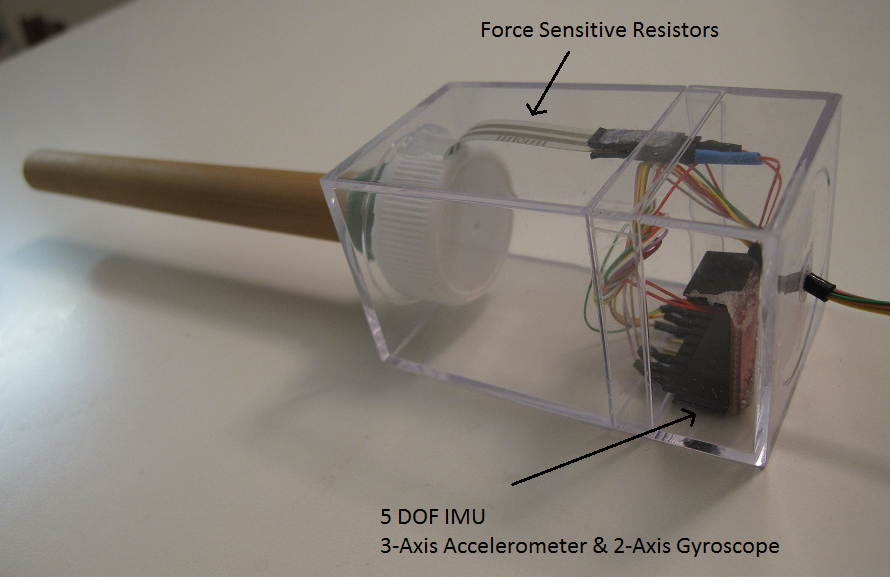
\includegraphics[width=\linewidth]{./figs/impl1.png}
  \caption{The Tangible Tube with all the sensors.}
  \label{fig:impl1}
\end{figure}


We have developed two applications to demonstrate the interactivity of our \tube. The applications that we developed are written in processing since it provides a smooth interface with arduino while boasting numerous easy-to-use graphical functions. Making existing processing applications to work with our \tube require very minimal changes to the code base since we have made the interface to the hardware to be very simple and generic.

% \subsection{Painting}
Our first application is a painting application program. In this application, the user will be able to paint by blowing into the tube and the harder the user blows, the thicker the color is. Changing the color of the paint is achieved by rotating the tube.

% \subsection{Shooting Game}
Our second application is a game in which the user is required to pass through a set of levels by shooting down balloons that randomly appear in the screen. This is done by moving the pointer to where the balloons are and blow into the tube. To make the game more interesting, the user will only be able to shoot down a particular balloon if the color of the pointer matches the color of that balloon. Similar to the previous application, changing the color of the pointer is done by rotating the tube.

\TODO
- Pictures \newline
- More details
